\subsection{In Databases}
The benefit of supporting vector search in DBMS is that this makes it easy to use for the end user and can be optimized for large datasets.

\subsection{Filtered Vector Search (FVS)}
This allows us to query both structured and unstructured data. In concept, this is SQL + Vectors, sometimes plus joins, subquery expressions,
multiple vector searches (on both sides of the join). Sometimes, the dataset isn't even a vector + tag stored in main memory.

Indices are typically built on unfiltered data. Thus, we need to think about the proper execution method. Suppose we are to retrieve $K$ rows with filtering:
\begin{itemize}
    \item \bi{Pre-Filter}: Filter first, then run \texttt{NNS}, and we get the $K$ rows. This is expensive if the filter is not selective.
    \item \bi{Post-Filter}: We first run \acrshort{ann} search, from which we get $K'$ rows which we then filter to get our $K$ rows.
          This is a recall and performance challenge, because if $K' \gg K$, then we have a lot of wasted effort.
          If on the other hand $K' > K$ and thus $\sigma(K') < K$, then we have low recall.
\end{itemize}

One way around this issue is to apply an \textit{inline filter}, i.e. during \acrshort{ann} search, we do vector search, evaluate the stopping condition and apply the filter.
This gives us $K$ rows directly and a handy performance uplift to go along with it.

Sounds too good to be true? That's because it is. There are still some issues, namely if filtered out nodes don't participate in the navigation.
In that case, the search stops if we reach such a filtered node, but there would be nodes that are closer to the query behind this node,
which due to the removal of the filtered out node are now no longer accessible.

This means that we need to have the filtered nodes participate in the navigation, which increases the cost by increasing the number of needed distance computations.

Thus, \textit{filters increase the search effort and difficulty of tuning search parameters}.
Selective filters make it harder to find valid nodes.

This is where the \texttt{Value-Vector-Correlation} comes in. It captures the relationship between the \bi{probability of satisfying the filters}
and the \bi{distance from the query vector}.
It doesn't however always correlate positively and the correlation depends on the query.
For instance, a query like ``Item like a blue T-Shirt and price > \$10K'' is negatively correlated.


\subsubsection{Hash-Tree Index}
If we use a Hash-Tree instead of the HNSW index, with filtering the internal node navigation does not change, as the data vectors are only in the leaves,
so we simply filter there.


\subsubsection{Performance Challenges}
The cost of a vector search is given by $f(n_d \cdot c_d, n_f \cdot c_f)$, where $n_d$ is the number of distance computations, $n_f$ is the number of filter evaluations
and $c_i$ and $c_f$ are the associated costs.

Depending on the query, the cost very much differs, in that for 20\% selectivity, filtering first is faster, while for 50\% selectivity, doing the NNS first is faster.

Since the distance computation and associated access costs are relative to the vector size,
we could use Principal Component Analysis (PCA) or others to reduce the dimension of the vectors.
Alternatively, we can quantize some values, with the drawback of reducing precision.
Trees offer more residualization, so the best of both worlds is to score fast with quantized vectors, then re-score with the full precision on just a subset.

A further optimization is to change how much of the set we re-score vs how much of it we score.

Not all dataset and query combinations are equally easy, and filters also change the difficulty.


\subsubsection{Filter agnosticism}
Filter agnosticism isn't just a single type, it's a spectrum.

\begin{figure}[h!]
    \begin{center}
        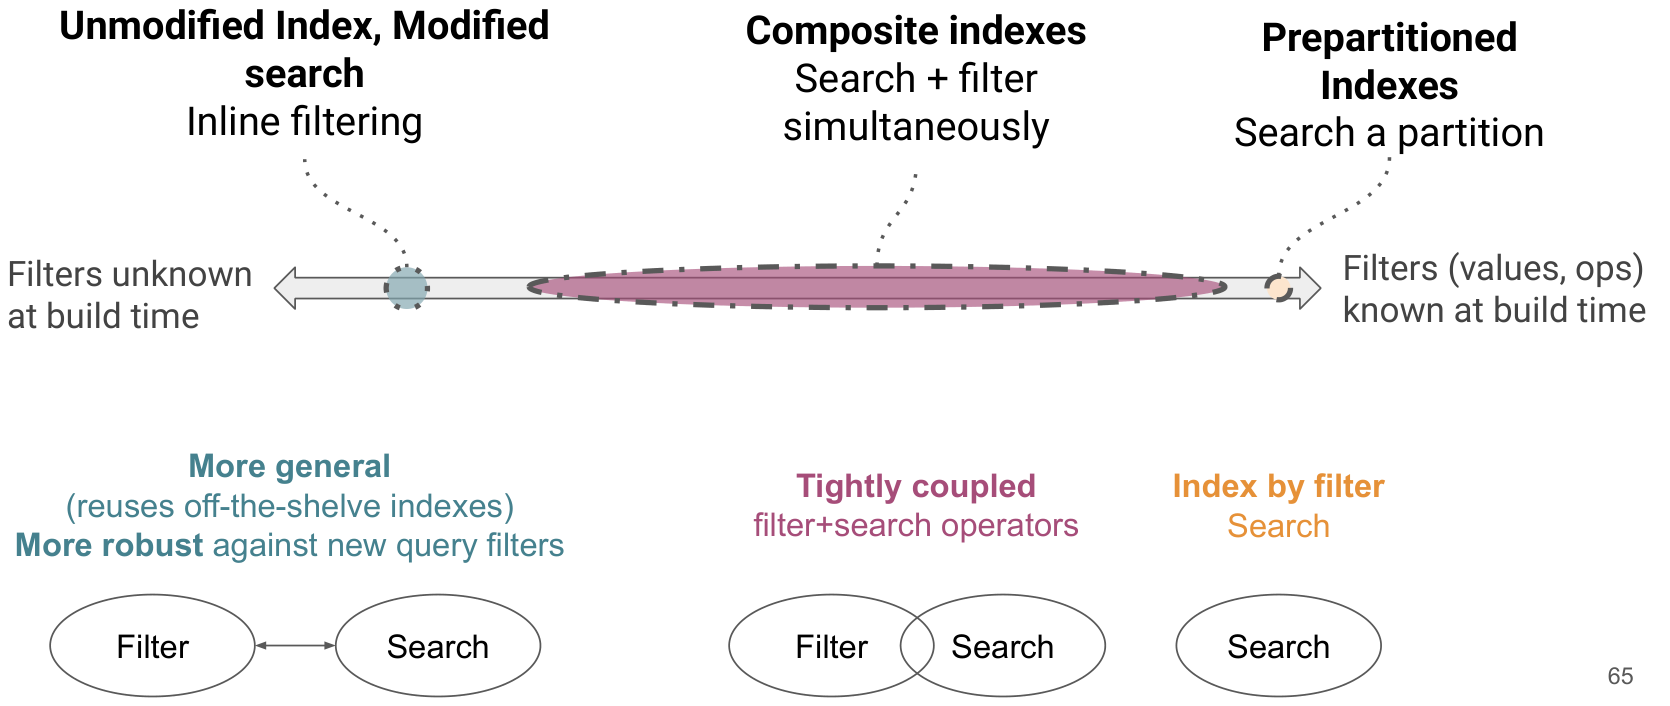
\includegraphics[width=0.8\textwidth]{assets/filter-agnosticism.png}
    \end{center}
    \caption{Spectrum of filter agnosticism
        (Figure from lecture slides 18, slide 65)}
\end{figure}

Ideally, we would build an index per filter, but there are issues:
\begin{itemize}
    \item Footprint is too high because of duplicated nodes
    \item Not enough data to build an index on the small partitions
\end{itemize}
We can emulate this partitioning with efficient footprint using a monolithic graph with pruning.

\inlinedefinition[Value-induced neighbourhood] We can build a new index based on attributes and embedding similarity (embedding distance)

\inlinedefinition[Predicate Traversal] Alternatively we can reuse unfiltered indexes and use inline filtering to discover filter-passing nodes,
then light up the right neighbourhood at search time.

\inlinedefinition[Densified Predicate Traversal] We also add edges to alleviate connectivity issues and proceed as with the predicate traversal
